\section{进程管理}

\begin{frame}[fragile]{CH2 进程管理}
  \begin{easylist} \easyitem
    & 2.1 进程的基本概念
    & 2.2 进程控制
    & 2.3 进程同步
    & 2.4 经典进程同步问题
    & 2.5 管程机制
    & 2.6 进程通信
    & 2.7 线程
  \end{easylist}
\end{frame}


\subsection{2.1 进程的基本概念}
\begin{frame}[fragile]{2.1 进程的基本概念}
  \begin{easylist} \easyitem
    & 未配置OS的系统:程序顺序执行
    && 程序的顺序执行及其特征
    & 现代多道程序环境下:程序并发执行
    && 程序的并发执行及其特征
  \end{easylist}
\end{frame}


\begin{frame}[fragile]{2.1 进程的基本概念}
  \begin{easylist} \easyitem
    & 2.1.1  程序的顺序执行及特征
    && 1. 程序执行有固定的时序
    \begin{center}
      \scalebox{0.7}{
        \begin{tikzpicture}[c/.style={draw,circle, thick, minimum height=0.5cm}]
          \draw[] node[c] (i1) {$I_1$}
          node[c, right=of i1] (c1) {$C_1$}
          node[c, right=of c1] (p1) {$P_1$}
          node[c, right=of p1] (i2) {$I_2$}
          node[c, right=of i2] (c2) {$C_2$}
          node[c, right=of c2] (p2) {$P_2$};
          \path[-Latex] (i1) edge (c1) (c1) edge (p1) (p1) edge (i2) (i2) edge (c2) (c2) edge (p2);
        \end{tikzpicture}
      }
    \end{center}

    && 2. 程序顺序执行时的特征
    &&& 顺序性:操作的前后依赖性
    &&& 封闭型:独占资源,资源状态只有本程序更改
    &&& 可再现性:初始环境和条件,结果相同
  \end{easylist}
\end{frame}


\begin{frame}[fragile]{程序顺序执行的优点}
  \begin{easylist} \easyitem
    & 符合人的直觉
    & 有利于错误调试
    && DEMO
    && BUG vs DEBUG
  \end{easylist}
  \begin{columns}[onlytextwidth,T]
    \begin{column}{0.5\textwidth}
      \begin{block}{\small 格蕾丝·赫柏(Grace Murray Hopper)}
        \scriptsize
        赫柏是一位为美国海军工作的电脑专家。1945年的一天,赫柏对Harvard Mark II设置好17000个继电器进行编程后,技术人员在进行整机运行时,它突然停止了工作。于是他们爬上去找原因,发现这台巨大的计算机内部一组继电器的触点之间有一只飞蛾,这显然是由于飞蛾受光和热的吸引,飞到了触点上,然后被高电压击死。所以在报告中,赫柏用胶条贴上飞蛾,并把“bug”来表示"一个在电脑程序里的错误"。
      \end{block}
    \end{column}
    \begin{column}{0.45\textwidth}
      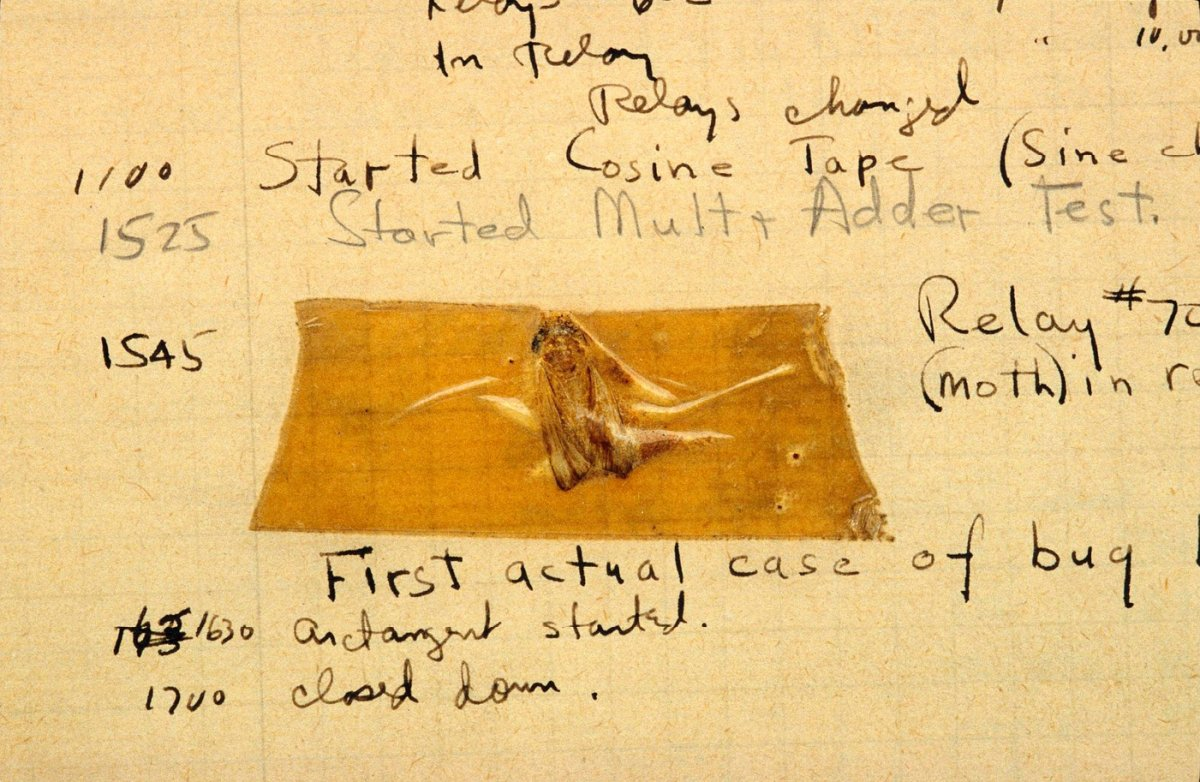
\includegraphics[width=0.85\textwidth]{figure/bug.jpg}
    \end{column}
  \end{columns}
\end{frame}


\begin{frame}[fragile]{2.1.2 程序的并发执行}
  \begin{easylist} \easyitem
    & 特征
    && 间断性:
    &&& 如打印程序等待计算程序完成之后方可继续
    &&& 执行—暂停—执行……
    && 失去封闭性
    &&& 主要由共享资源引起,资源的状态将由多个程序改变;
    && 不可再现性
    &&& 计算结果与并发程序的执行速度有关
  \end{easylist}
\end{frame}


\begin{frame}[fragile]{例子 --- 课堂讨论}
  \begin{easylist} \easyitem
    & 有2个循环程序$A$和$B$,共享一个变量$N$( 设$N$的初值为$n$ )
    & 程序$A$每执行一次时,都要做$N:=N+1$
    & 程序$B$每次要执行$Print(N)$, 然后再做$N:=0$
    \vspace{1cm}
    & 若程序$A$,$B$以不同的速度运行,其结果将会是?
    & 注意,代码采用了类Pascal语言
  \end{easylist}
\end{frame}


\begin{frame}[fragile]{例子}
  \begin{easylist} \easyitem
    & N:=N+1在print(N)和N:=0之前,则N值分别为n+1, n+1, 0.
    & N:=N+1在print(N)和N:=0之后,则N值分别为n, 0, 1.
    & N:=N+1在print(N)和N:=0之间,则N值分别为n, n+1, 0.
  \end{easylist}
\end{frame}


\begin{frame}[fragile]{Python代码示例}
  \begin{lstlisting}[keywordstyle=\color{red},basicstyle=\small, language=python]
from multiprocessing import Process
def f1(i):
    while i<10:
        i = i+1
    print 'f1 finished‘

def f2(i):
    while i>-10:
        i = i-1
    print 'f2 finished!'


if __name__=='__main__':
    Process(target=f1, args=(0,)).start()
    Process(target=f2, args=(0,)).start()
\end{lstlisting}
\end{frame}


\begin{frame}[fragile]{多次运行结果}
  \begin{easylist} \easyitem
    & Run 1:
    && f1 finished
    && f2 finished!
    & Run 2:
    && f1 finished
    && f2 finished!
    & Run 3:
    && f2 finished!
    && f1 finished
  \end{easylist}
\end{frame}


\begin{frame}[fragile]{思考}
  \begin{easylist} \easyitem
    & 在多道程序环境下,程序执行属于并发执行,具有3个典型特性(哪3个?)
    & 结果的不可再现性的问题
    & 要保证结果的再现性,就需要对并发执行的程序加以描述和控制,其结果就是引入了“进程”概念
    & 进程=程序+执行
    & 在Multics OS之前,主要采用IBM的“作业(job)”概念,之后,改为进程(Process)
  \end{easylist}
\end{frame}


\subsection{2.1.3 进程的特征和状态}
\begin{frame}[fragile]{2.1.3 进程的特征和状态}
  \begin{easylist} \easyitem
    & 进程的定义
    && 程序的一次执行过程
    && 进程是程序实体的执行过程,是系统进行资源分配与调度的独立单位。
  \end{easylist}
\end{frame}


\begin{frame}[fragile]{进程的特征}
  \begin{easylist} \easyitem
    & 1.结构特征
    && 进程:由程序段、数据段及进程控制块三部分构成,总称“进程映像(Unix中)”。
    & 2.动态性:进程实体的一次执行过程
    && 由“创建”而产生,由“调度”而执行;由得不到资源而阻塞;由撤消而消亡。(而程序是静态的)。
    & 3.并发性:只有建立了进程,才能并发执行
    && 如同时浏览多个网页
    & 4.独立性: 独立运行,独立获得资源。资源分配与调度的基本单位
    && 浏览器邮箱登陆实例
    & 5.异步性:
    && 各进程以不可预知的速度向前推进
    && 间断性
  \end{easylist}
\end{frame}


\begin{frame}[fragile]{进程的状态}
  \begin{easylist} \easyitem
    & 进程执行的间断性,使得进程具有多种不同的状态
    & 进程的三种基本状态
    && 就绪
    && 执行
    && 阻塞
  \end{easylist}
  \vspace*{-1cm}
  \centering
  \begin{figure}
    \begin{tikzpicture}[c/.style={draw,ellipse, thick, minimum height=0.5cm}]
      \draw[] node[c] (ready) {就绪}
      node[c, below left=of ready, xshift=-1cm] (block) {阻塞}
      node[c, fill=yellow!50, below right=of ready, yshift=-1cm] (exec) {执行};

      \path[->,thick] (block) edge[bend left=30] node[below right]{I/O完成} (ready)
      (exec) edge[bend left=30] node[below]{I/O请求} (block)
      (ready) edge[bend right=30] node[left]{进程调度} (exec)
      (exec) edge[bend right=30] node[right]{时间片完} (ready);
    \end{tikzpicture}
    \caption{进程的三种基本状态及其转换}
  \end{figure}
\end{frame}


\begin{frame}[fragile]{挂起状态(被换出内存的状态)}
  \begin{easylist} \easyitem
    & 引入原因
    && 终端用户请求
    && 父进程请求
    && 负荷调节需要
    && 操作系统需要
    & 挂起演示
    && vi,CTRL+z; debugging
    & 进程状态的转换
    && 活动就绪 $\Rightarrow$ 静止就绪
    && 活动阻塞 $\Rightarrow$ 静止阻塞
    && 静止就绪 $\Rightarrow$ 活动就绪
    && 静止阻塞 $\Rightarrow$ 活动阻塞
  \end{easylist}
\end{frame}


\begin{frame}[fragile]{具有挂起状态的进程状态图}
\centering
\begin{figure}
  \scalebox{0.8}{
    \begin{tikzpicture}[c/.style={draw,ellipse, thick, minimum height=1cm, minimum width=2cm}]
      \draw[] node[c, fill=yellow!50] (exec) {执行}
      node[c, below left=1.5cm of exec, yshift=-1cm] (ready1) {活动就绪}
      node[c, below right=1.5cm of exec, yshift=-1cm] (ready2) {静止就绪}
      node[c, below left=1cm of ready1, yshift=-1cm] (block1) {活动阻塞}
      node[c, below left=1cm of ready2, yshift=-1cm, xshift=1cm] (block2) {静止阻塞};

      \path[->,thick] (exec) edge[bend left=10] (ready1) (ready1) edge[bend left=15] (exec)
      (exec) edge[bend left=30] node[right]{挂起} (ready2)
      (ready1) edge[bend right=30] node[above]{挂起} (ready2)
      (ready2) edge[bend right=15] node[above]{激活} (ready1)
      (exec) edge[bend right=40] node{请求I/O} (block1)
      (block1) edge[bend right=30] node[above]{挂起} (block2)
      (block2) edge[bend right=15] node[above]{激活} (block1)
      (block2) edge[bend right=15] node[right]{释放} (ready2)
      (block1) edge[bend left=15] node[right]{释放} (ready1);
    \end{tikzpicture}
  }
  \caption{具有挂起状态的进程状态及其转换}
\end{figure}
\end{frame}


\begin{frame}[fragile]{实验}
  \begin{easylist} \easyitem
    & 写一个程序描述进程状态迁移过程。
    & 要求:
    && 提供导致进程状态变化的调用接口,包括创建、删除、调度、阻塞、时间到、挂起、激活等。
    && 实现进程列表显示的接口。
    && 注:这里设计的进程是一个假设的对象实体,是由程序自己创建和删除,不是系统维护的进程。
  \end{easylist}
\end{frame}




\subsection{进程控制块}
\begin{frame}[fragile]{2.1.4 进程控制块}
  \begin{columns}[onlytextwidth,T]
    \begin{column}{0.7\textwidth}
      \begin{enumerate}
      \item 进程控制块的作用
        \begin{itemize}
        \item 使不能独立运行的程序变为能独立运行的基本单位
        \item 是进程存在的唯一标志
        \item PCB (Process Control Block)常驻内存
        \end{itemize}
      \item 进程控制块中的信息
        \begin{itemize}
        \item 标识、处理机状态,进程调度信息,进程控制信息
        \end{itemize}
      \end{enumerate}
    \end{column}
    \begin{column}{0.3\textwidth}
      \begin{tabular}{|c|}
        \hline
        pid \\ \hline
        进程状态 \\ \hline
        现场  \\ \hline
        优先级  \\ \hline
        阻塞原因  \\ \hline
        程序地址  \\ \hline
        同步机制  \\ \hline
        资源清单  \\ \hline
        链接指针  \\ \hline
      \end{tabular}
    \end{column}
  \end{columns}
\end{frame}


\begin{frame}[fragile]{PCB}
  \begin{easylist} \easyitem
    & 进程标识符
    && 内部标识符与外部标识符(下页top示例)
    & 处理机状态
    && 能在断点恢复运行
    && 通用寄存器、指令计数器、程序状态字PSW、用户栈指针
    & 进程调度信息
    && 进程状态、优先级、与调度有关的其他信息(如等待时间)、事件(阻塞事件)
    & 进程控制信息
    && 程序和数据的地址
    && 进程同步和通信机制:消息队列指针、信号量
    && 资源清单
    && 在PCB队列中的链接指针
  \end{easylist}
\end{frame}

\begin{frame}[fragile]
  \frametitle{Linux top command}
  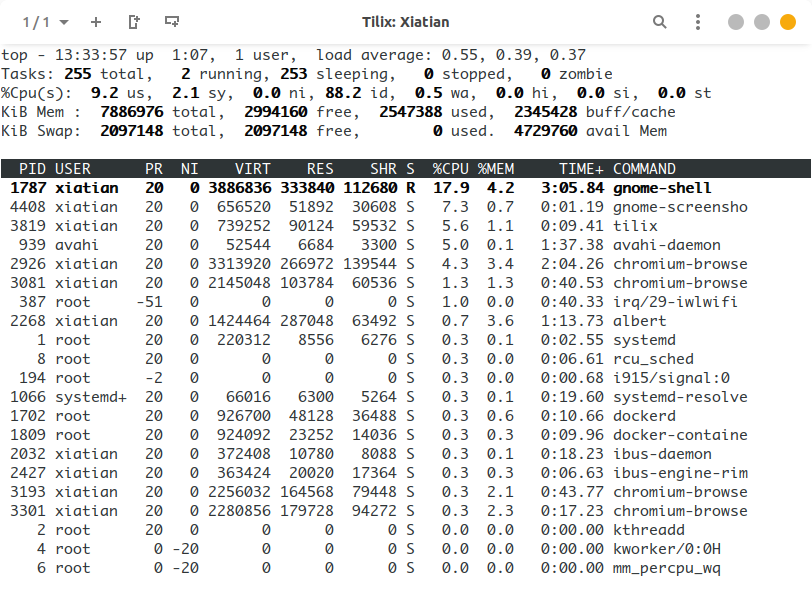
\includegraphics[width=0.9\textwidth]{figure/process-top.png}
\end{frame}



\begin{frame}[fragile]{PCB的组织: 链接方式}
  \centering
  \begin{figure}
    \scalebox{0.8}{
      \begin{tikzpicture}[q/.style={draw,thick, minimum height=0.8cm, minimum width=2.5cm},
        b/.style={draw, minimum width=1.5cm, minimum height=0.8cm}]
        \draw node[q] (exec) {执行指针} node[q, below=of exec] (ready) {就绪队列指针} node[q, below=of ready] (block) {阻塞队列指针} node[q, below=of block] (free) {空闲队列指针};

        \draw node[b, above right=3cm of exec, yshift=-1cm] (p1) {PCB1} node[b, right=0 of p1] (l1) {4};
        \draw node[b, below=0 of p1] (p2) {PCB2} node[b, right=0 of p2] (l2) {3};
        \draw node[b, below=0 of p2] (p3) {PCB3} node[b, right=0 of p3] (l3) {$\wedge$};
        \draw node[b, below=0 of p3] (p4) {PCB4} node[b, right=0 of p4] (l4) {8};
        \draw node[b, below=0 of p4] (p5) {PCB5} node[b, right=0 of p5] (l5) {$\wedge$};
        \draw node[b, below=0 of p5] (p6) {PCB6} node[b, right=0 of p6] (l6) {7};
        \draw node[b, below=0 of p6] (p7) {PCB7} node[b, right=0 of p7] (l7) {9};
        \draw node[b, below=0 of p7] (p8) {PCB8} node[b, right=0 of p8] (l8) {0};
        \draw node[b, below=0 of p8] (p9) {PCB9} node[b, right=0 of p9] (l9) {$\wedge$};
        \draw node[b, below=0 of p9] (p10) {$\cdots$} node[b, right=0 of p10] (l10) {$\cdots$};

        \path[->, thick] (l1.east) edge[draw=blue, to path={-- ++(1,0) |- (\tikztotarget)}] (l4.east);
        \path[->, thick] (l2.east) edge[draw=orange, to path={-- ++(0.5,0) |- (\tikztotarget)}] (l3.east);
        \path[->, thick] (l4.east) edge[draw=blue, to path={-- ++(0,-0.2)-- ++(1,0) |- (\tikztotarget)}] (l8.east);

        \path[->, thick] (l6.east) edge[draw=purple, to path={-- ++(0,-0.2)-- ++(0.5,0) |- (\tikztotarget)}] (l7.east);
        \path[->, thick] (l7.east) edge[draw=purple, to path={-- ++(0,-0.2)-- ++(0.5,0) |- (\tikztotarget)}] (l9.east);

        \draw[->, thick] (exec.east)--(p5.west);
        \draw[->, thick, draw=blue] (ready.east)--(p1.west);
        \draw[->, thick, draw=orange] (block.east)--(p2.west);
        \draw[->, thick, draw=purple] (free.east)--(p6.west);
      \end{tikzpicture}
    }
    \caption{PCB链接组织方式}
  \end{figure}
\end{frame}


\begin{frame}[fragile]{PCB的组织: 索引方式}
  \centering
  \begin{figure}
    \scalebox{0.8}{
      \begin{tikzpicture}[q/.style={draw,thick, minimum height=0.8cm, minimum width=2.5cm},
        a/.style={draw, -latex}]
        \draw node[q, fill=yellow!20] (exec) {执行指针} node[q, below=of exec] (ready) {就绪表指针} node[q, below=of ready] (block) {阻塞表指针};

        \draw node[q, minimum height=0.6cm, above right=of exec,yshift=-1cm] (rlist1) {} node[q, minimum height=0.6cm, below=0 of rlist1] (rlist2) {} node[q, minimum height=0.6cm, below=0 of rlist2] (rlist3) {} node[q, minimum height=0.6cm, below=0 of rlist3] (rlist4) {};

        \draw node[q, minimum height=0.6cm, below=of rlist4] (blist1) {} node[q, minimum height=0.6cm, below=0 of blist1] (blist2) {} node[q, minimum height=0.6cm, below=0 of blist2] (blist3) {} node[q, minimum height=0.6cm, below=0 of blist3] (blist4) {};

        \draw node[q, above right=1.5cm of rlist1, yshift=-1cm] (pcb1) {PCB1}
        node[q, below=0 of pcb1] (pcb2) {PCB2}
        node[q, below=0 of pcb2] (pcb3) {PCB3}
        node[q, below=0 of pcb3] (pcb4) {PCB4}
        node[q, below=0 of pcb4] (pcb5) {PCB5}
        node[q, below=0 of pcb5] (pcb6) {PCB6}
        node[q, below=0 of pcb6] (pcb7) {PCB7}
        node[q, below=0 of pcb7,draw=white] (pcb8) {$\cdots$};

        \path[a] (exec.east) edge[bend left=40] (pcb1.west);
        \draw[a] (ready.east)--(rlist1.west);
        \draw[a] (block.east)--(blist1.west);

        \draw[a] (rlist1.east)--(pcb3.west);
        \draw[a] (rlist2.east)--(pcb2.west);
        \draw[a] (rlist3.east)--(pcb4.west);

        \draw[a] (blist1.east)--(pcb7.west);
        \draw[a] (blist2.east)--(pcb6.west);
        \draw[a] (blist3.east)--(pcb5.west);
      \end{tikzpicture}
    }
    \caption{PCB索引组织方式}
  \end{figure}
\end{frame}

\begin{frame}[fragile]{补充}
  \begin{easylist} \easyitem
    & 指针和链表的概念
    && E.g.从链表中移除我的下一个:
    &&& 我的下一个是(变成)我的下一个的下一个
    && E.g. 从链表中移除我本身
    &&& 我的上一个的下一个是我的下一个

    & PCB和进程的代码数据放在一起吗?
    && 系统态和用户态
    && 系统空间和用户空间

    & 系统调用和普通调用的区别?
    && 系统调用会引起从用户态进入核心态
  \end{easylist}
\end{frame}

\begin{frame}[fragile]{Review last lesson}
  \begin{easylist} \easyitem
    & 什么是PCB,操作系统采用哪些方式对PCB进行组织和管理的?
  \end{easylist}
\end{frame}

\subsection{2.2 进程控制}
\begin{frame}[fragile]{2.2 进程控制}
  \begin{easylist} \easyitem
    & 2.2.1 进程的创建
    & 2.2.2 进程的终止
    & 2.2.3 进程的阻塞与唤醒
    & 2.2.4 进程的挂起与激活
  \end{easylist}
\end{frame}


\begin{frame}[fragile]{2.2.1 进程的创建}
  \begin{easylist} \easyitem
    & 进程图:
    & 引起创建进程的事件:
    & 进程的创建
  \end{easylist}
\end{frame}


\begin{frame}[fragile]{进程图}
  \begin{easylist} \easyitem
    && 描述了进程的家族关系
    && 子进程可继承父的资源,撤消时应归还给父进程,父的撤消会撤消全部子进程。
  \end{easylist}
\end{frame}


\begin{frame}[fragile]{引起创建进程的事件}
  \begin{easylist} \easyitem
    && 1.用户登录:
    &&& 为终端用户建立一进程
    && 2.作业调度:
    &&& 为被调度的作业建立进程
    && 3.提供服务:
    &&& 如要打印时建立打印进程
    && 4.应用请求:
    &&& 由应用程序建立多个进程
  \end{easylist}
\end{frame}


\begin{frame}[fragile]{进程的创建}
  \begin{easylist} \easyitem
    & (create原语)
    && 1.申请空白PCB(一个系统的PCB是有限的)
    && 2.为新进程分配资源(不同于一般的分配,PCB-LIST在一个特殊区域)
    && 3.初始化PCB
    && 4.将新进程插入就绪队列。
  \end{easylist}
\end{frame}


\begin{frame}[fragile]{2.2.2 进程的终止}
  \begin{easylist} \easyitem
    & 引起进程终止的事件
    & 进程的终止过程
  \end{easylist}
\end{frame}

\begin{frame}[fragile]{引起进程终止的事件}
  \begin{easylist} \easyitem
    & 1. 正常结束:如Halt、logoff
    & 2. 异常结束:如Protect error、overtime等
    & 3. 外界干预:
    && a. 系统员kill进程;(Linux演示)
    && b. 父进程终止;(impressive打开pdf文件演示)
    && c. 父进程请求。
  \end{easylist}
\end{frame}

\begin{frame}[fragile]{进程的终止过程}
  \begin{easylist} \easyitem
    & 1. 检查进程状态;
    & 2. 执行态$\rightarrow$中止,且置调度标志为真。
    & 3. 有无子孙需终止。
    & 4. 归还资源给其父进程或系统。
    & 5. 从PCB队列中移出PCB.
  \end{easylist}
\end{frame}



\begin{frame}[fragile]{2.2.3 进程的阻塞与唤醒}
  \begin{easylist} \easyitem
    & Content:
    && 引起进程阻塞和唤醒的事件
    && 进程阻塞过程
    && 进程唤醒过程
  \end{easylist}
\end{frame}

\begin{frame}[fragile]{引起进程阻塞和唤醒的事件}
  \begin{easylist} \easyitem
    & 1.请求系统服务而得不到满足时,如向系统请求打印。
    & 2.启动某种操作而需同步时:如该操作和请求该操作的进程需同步运行(即非异步操作)。
    & 3.新数据尚未到达:如进程A写,进程B读,则A未写完B不能读。
    & 4.无新工作可做。
  \end{easylist}
\end{frame}

\begin{frame}[fragile]{阻塞过程}
  \begin{easylist} \easyitem
    & 是进程自身的一种主动行为
    && a.调block原语
    && b.停止执行,修改PCB入阻塞队列(一个或多个),并转调度。
  \end{easylist}
\end{frame}

\begin{frame}[fragile]{唤醒过程}
  \begin{easylist} \easyitem
    & 其它相关进程完成。
    && a.wakeup原语
    && b.修改PCB,入就绪队列
    && 可见,有block原语,在其它进程中就应有wakeup原语。
  \end{easylist}
\end{frame}

\begin{frame}[fragile]{2.2.4 进程的挂起与激活}
   \begin{easylist} \easyitem
    & 进程的挂起过程
    && 由进程自己或其父进程调suspend原语完成,将该进程PCB移到指定区域,注意状态的改变,有可能要重新调度。
    & 进程的激活过程。
    && active原语(如在外存,调入内存,改变状态,根据情况看是否调度,如抢先或非抢先)。
    \vspace{1cm}
    & 阻塞、唤醒一般由OS实现,而挂起与激活可由用户干预。
  \end{easylist}
\end{frame}


\subsection{2.3 进程同步}
\begin{frame}[fragile]{2.3 进程同步}
  \begin{easylist} \easyitem
    & 并发提高了资源利用率和系统吞吐量,但也会给系统造成混乱。
    & 同步:
    && 并发进程在执行次序上的协调,以达到有效的资源共享和相互合作,使程序执行有可再现性。
  \end{easylist}
\end{frame}

\begin{frame}[fragile]{2.3.1 进程同步的基本概念}
  \begin{easylist} \easyitem
    & 1.两种形式的制约关系
    && 资源共享关系:(进程间接制约)
    &&& 如争用一台打印机
    &&& 需互斥地访问临界资源。
    && 相互合作关系:(进程直接制约)
    &&& 如A的输出作为B的输入
    &&& 需要同步解决
    & 2. 临界资源:(一次仅允许一个进程访问的资源)
    && 引起不可再现性是因为临界资源没有互斥访问。
  \end{easylist}
\end{frame}

\begin{frame}[fragile]{生产者-消费者问题}
  \begin{lstlisting}[tabsize=8,keywordstyle=\color{red},basicstyle=\small, language=Pascal, numbers=none]
var n, integer;  //变量定义
Type item=…;
var buffer:array[0,1,…,n-1] of item;
in, out: 0,1, …, n-1;
counter: 0,1,…,n;
    \end{lstlisting}
\end{frame}

\begin{frame}[fragile]{生产者-消费者问题}
  \begin{columns}[onlytextwidth,T]
    \begin{column}{0.48\textwidth}
      \begin{lstlisting}[tabsize=8,keywordstyle=\color{red},basicstyle=\small, language=Pascal]
producer:
repeat
      produce an item in nextp;
      …
      while counter=n do no-op;
      buffer[in]:=nextp;
      in:=(in+1)mod n;
      counter:=counter+1;
until false; \end{lstlisting}
    \end{column}
    \begin{column}{0.5\textwidth}
      \begin{lstlisting}[tabsize=8,keywordstyle=\color{red},basicstyle=\small, language=Pascal]
consumer:
repeat
        while counter=0 do no-op;
        nextc:=buffer[out];
        out:=(out+1) mod n;
        counter:=counter-1;
        consumer the item in nextc;
until false; \end{lstlisting}
    \end{column}
  \end{columns}
\end{frame}


\begin{frame}[fragile]{Question}
  \begin{easylist} \easyitem
    & 两个进程共享变量counter
    & counter会导致结果不确定
  \end{easylist}
\end{frame}

\begin{frame}[fragile]{生产者-消费者问题(2)}
  \begin{easylist} \easyitem
    & 设counter的初值为5
  \end{easylist}

  \begin{columns}[onlytextwidth,T]
    \begin{column}{0.4\textwidth}
      \begin{lstlisting}[tabsize=8,keywordstyle=\color{red},basicstyle=\small, language=Pascal, numbers=none]
register1:=counter;
register1 :=register1+1;
counter :=register1;    \end{lstlisting}
    \end{column}
    \begin{column}{0.4\textwidth}
      \begin{lstlisting}[tabsize=8,keywordstyle=\color{red},basicstyle=\small, language=Pascal, numbers=none]
register2:=counter;
register2:=register2-1;
counter :=register2;      \end{lstlisting}
    \end{column}
  \end{columns}

\begin{tabular}{l l }
  register1:=counter;        &    (register1:=5) \\
  register1 :=register1+1;   &    (register1:=6) \\
  register2:=counter;        &	  (register2:=5) \\
  register2 :=register2-1;   &	  (register2:=4) \\
  counter :=register1;       &    (counter:=6) \\
  counter :=register2;       &    (counter:=4) \\
\end{tabular}
\end{frame}


\begin{frame}[fragile]{3. 临界区}
  \begin{easylist} \easyitem
& 定义:进程访问临界资源的那段代码称为临界区
& 访问临界资源的描述:
&& 进入区:检查有无进程进入
&& 临界区:
&& 退出区:将访问标志复位
  \end{easylist}

  \begin{lstlisting}[tabsize=8,keywordstyle=\color{red},basicstyle=\small, language=Pascal]
Repeat
    Entry section
    Critical section
    Exit section
Until false \end{lstlisting}
\end{frame}

\begin{frame}[fragile]{4. 同步机制应遵循的准则}
  \begin{easylist} \easyitem
    & 1.空闲让进
    & 2.忙则等待
    & 3.有限等待
    && 应保证为有限等待,避免“死等”。
    & 4.让权等待
    && 不能进入临界区的执行进程应放弃CPU执行权。避免“忙等”
  \end{easylist}
\end{frame}

\begin{frame}[fragile]{2.3.2 信号量机制}
  \begin{easylist} \easyitem
    & Edsger Wybe Dijkstra(1930年5月11日--2002年8月6日)
    && 毕业于Leiden大学
    && 1972年获得图灵奖
    && 1989年计算机科学教育杰出贡献奖
    && 2002年ACM PODC最具影响力论文奖
    & 与Knuth并称为我们这个时代最伟大的计算机科学家的人。
    && 提出“goto有害论”;
    && 1965年,{\color{red} 提出信号量和PV原语};
    && 解决了有趣的{\color{red}“哲学家聚餐”}问题;
    &&  最短路径算法(SPF)和{\color{red}银行家算法}的创造者;
    && 第一个Algol 60编译器的设计者和实现者;
    && THE操作系统的设计者和开发者;
  \end{easylist}

  \begin{picture} (0,0)
    \put(260,30){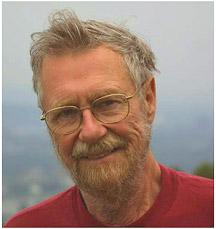
\includegraphics[width=0.25\textwidth]{figure/dijkstra.jpg}}
  \end{picture}
\end{frame}

\begin{frame}[fragile]{2.3.2 信号量机制}
  \begin{easylist} \easyitem
& 1 整型信号量
&& 是一个整型量,通过2个{\color{red}原子操作}wait(s)和signal(s)来访问。
&& Wait(s):
\begin{lstlisting}[tabsize=8,keywordstyle=\color{red},basicstyle=\small, language=Pascal, numbers=none]
while s<= 0 do no-op;
s:=s-1;
\end{lstlisting}
&& Signal(s):
\begin{lstlisting}[tabsize=8,keywordstyle=\color{red},basicstyle=\small, language=Pascal, numbers=none]
s:=s+1;
\end{lstlisting}
  \end{easylist}
\end{frame}



\begin{frame}[fragile]{2 记录型信号量}
\begin{columns}[onlytextwidth,T]
    \begin{column}{0.6 \textwidth}
\begin{lstlisting}[tabsize=8,keywordstyle=\color{red},basicstyle=\small, language=Pascal]
type  semaphore=record
        value:integer;
        L: list of process;
end
procedure wait(s)
  var s: semaphore
  begin
        s.value:=s.value - 1;
        if s.value < 0 then block (s, L)
  end
procedure signal (s)
  var s:semaphone
  begin
        s.value:=s.vaule + 1
        if s.value<=0 then wakeup(s.L)
  end
\end{lstlisting}
\end{column}
\begin{column}{0.4\textwidth}
  \small
  \begin{itemize}
  \item L:为进程链表,用于链接所有等待该类资源进程。
  \item 用wait(s)和signal(s)实现同步与互斥。
  \item 在记录型信号量机制中:
  \item s.value初值:表示系统中某类资源的数目。
  \item s.value<0:表该信号量链表中已阻塞进程的数目。
  \item Qestion: 为什么叫“记录型”信号量?
  \end{itemize}
\end{column}
\end{columns}

\end{frame}


\begin{frame}[fragile]{PV操作}
  \begin{easylist} \easyitem
    & Wait(s): 也用$P(s)$或者$Down(s)$ 表示,相当于申请资源
    & Signal(s): 也用$V(s)$ 或者$Up(s)$ 表示,相当于释放资源
    & 例如:
    && 在公共电话厅打电话
  \end{easylist}
\end{frame}


\begin{frame}[fragile]{3 AND型信号量}
  \begin{easylist} \easyitem
    & 当不用它时,有可能发生系统死锁。
    & 死锁:在无外力作用下的一种僵持状态。
    & 特点:要么全分配,要么一个也不分配。
  \end{easylist}
\end{frame}


\begin{frame}[fragile]{3 AND型信号量}
  \centering
  \begin{tabular}{| l | l |}
    \hline
    process A: & process B: \\
    wait(Dmutex); & wait(Emutex); \\
    wait(Emutex);~~~~~~ & wait(Dmutex);~~~~~~~ \\
    \hline
  \end{tabular}

  \vspace{2cm}
  若两个进程交替执行,则死锁
\end{frame}



\begin{frame}[fragile]{3 AND型信号量}
\begin{lstlisting}[tabsize=8,keywordstyle=\color{red},basicstyle=\small, language=Pascal]
Swait(s1,s2,…,sn)
    if s1 >= 1 and … and sn >= 1 then
        for i:=1 to n do si:=si-1; endfor
    else
        place the process in the waiting queue with the first si found    with si<1, and set the program count of this process to the beginning of swait operation
    end if

Ssignal(s1,s2,…,sn)
    for i:=1 to n do si:=si+1;

    remove all the process waiting in the queue associated with si into the ready queue
 endfor
\end{lstlisting}
\end{frame}

\begin{frame}[fragile]{4 信号量集}
  \begin{easylist} \easyitem
    & 某进程需要100个临界资源X时:
    && wait(x);
    && ……
    && wait(x)
    & 有些情况下,只有系统空闲资源数量大于等于一定数值,才予以分配。
  \end{easylist}
\end{frame}


\begin{frame}[fragile]{4 信号量集}
  \begin{easylist} \easyitem
    & 为提高效率而对AND信号的扩充。
    && Swait(S, t, d): t为下限制,d为需求值
    & 三种特例:
    && (1)Swait(S,d,d):允许每次申请d个资源。
    &&& 当资源数少于d时,不予分配。
    && (2)Swait (S,1,1):$S>1$,记录型信号量。
    &&& S=1时,互斥型信号量。
    && (3)Swait(S,1,0),可控开关,当$S \geq 1$时,允许进入,$S<1$时,不能进入。
  \end{easylist}
\end{frame}


\begin{frame}[fragile]{利用信号量实现互斥}
\begin{columns}[onlytextwidth,T]
\begin{column}{0.46 \textwidth}
\begin{lstlisting}[tabsize=8,keywordstyle=\color{red},basicstyle=\small, language=Pascal]
var mutex: semaphore:=1

parbegin
    process1:begin
        repeat
           wait(mutex);
           critical setion
           signal(mutex);
           remainder section
        until false;
    end
\end{lstlisting}
\end{column}
\begin{column}{0.46 \textwidth}
\begin{lstlisting}[tabsize=8,keywordstyle=\color{red},basicstyle=\small, language=Pascal, firstnumber=last]
    process2: begin
        repeat
           wait(mutex);
           critical setion
           signal(mutex);
           remainder section
        until false;
    end
parend
\end{lstlisting}
\end{column}
\end{columns}
\end{frame}


\subsection{2.4 经典进程同步问题}
\begin{frame}[fragile]{2.4 经典进程同步问题}
  \begin{easylist} \easyitem
    && 2.4.1 生产者—消费者问题
    && 2.4.2 哲学家进餐问题
    && 2.4.3 读者—写者问题
  \end{easylist}
\end{frame}

\begin{frame}[fragile]{生产者—消费者问题}
  \centering
  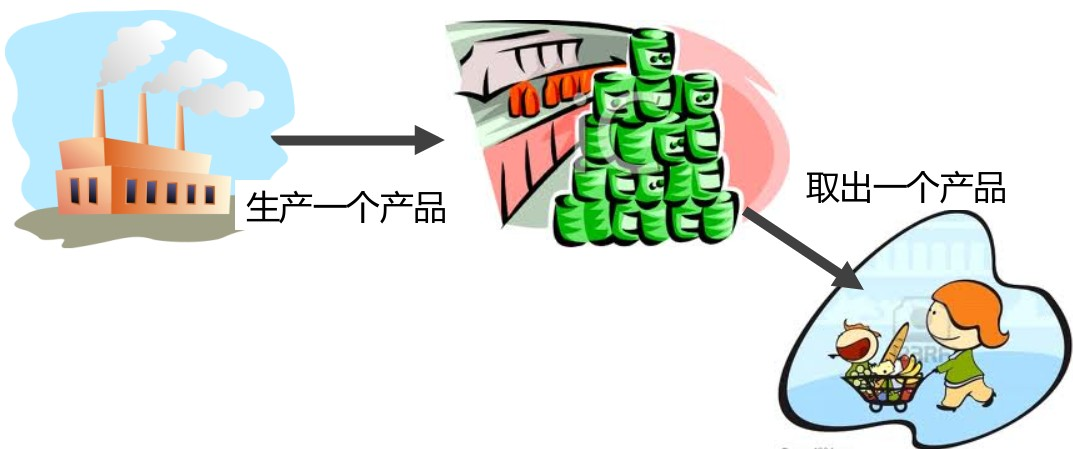
\includegraphics[width=0.85\textwidth]{figure/producer_consumer.jpg}
\end{frame}


\begin{frame}[fragile]{生产者—消费者问题}
  \begin{easylist} \easyitem
   & 定义两个同步信号量:
   && empty---表示缓冲区中空缓冲区的数量,初值为n(n个缓冲区)。
   && full---表示缓冲区中满的数量,初值为0。
   && mutex---使诸进程互斥地访问缓冲区
  \end{easylist}
\end{frame}


\begin{frame}[fragile]{记录型信号量解决生产者—消费者问题}
 \begin{lstlisting}[tabsize=8,keywordstyle=\color{red},basicstyle=\small, language=Pascal]
   var mutex,empty,full:Semaphore:=1,n,0;
       buffer:array[0,1,…,n-1] of item;
       in, out: integer: =0,0;
\end{lstlisting}
 
 \begin{columns}[onlytextwidth,T]
 \begin{column}{0.46 \textwidth}
 \begin{lstlisting}[tabsize=8,keywordstyle=\color{red},basicstyle=\small, language=Pascal, firstnumber=last, escapechar=|]
 producer: begin
     repeat
         …
         Produce an item in nextp;
         wait(empty);
         wait(mutex);
         buffer(in):=nextp;
         in:=(in+1) mod n;
         signal(mutex);
         signal(full);
     until false;
 end
 \end{lstlisting}
 \end{column} 
 \begin{column}{0.46 \textwidth}
 \begin{lstlisting}[tabsize=8,keywordstyle=\color{red},basicstyle=\small, language=Pascal, firstnumber=last, escapechar=|]
 consumer:begin
     repeat
         wait(full);
         wait(mutex);
         nextc:=buffer(out);
         out:=(out+1) mod n;
         signal(mutex);
         signal(empty);
         Consumer the item in nextc;
     until false;
 end
 \end{lstlisting}
 \end{column}
 \end{columns}
\end{frame}


 \begin{frame}[fragile]{利用AND信号量解决生产者—消费者问题}
 \begin{lstlisting}[tabsize=8,keywordstyle=\color{red},basicstyle=\small, language=Pascal]
 var  mutex, empty, full: semaphore:=1,n,0;
      buffer:array[0,…,n-1] of item;
      in out: integer :=0,0;
 \end{lstlisting}

 \begin{columns}[onlytextwidth,T]
 \begin{column}{0.46 \textwidth}
 \begin{lstlisting}[tabsize=8,keywordstyle=\color{red},basicstyle=\small, language=Pascal, firstnumber=last]
 producer: begin
     repeat
         …
         Produce an item in nextp;
         Swait(empty, mutex);
         buffer(in):=nextp;
         in:=(in+1) mod n;
         Ssingal(mutex, full);
     until false;
 end
 \end{lstlisting}
 \end{column}
 \begin{column}{0.46 \textwidth}
 \begin{lstlisting}[tabsize=8,keywordstyle=\color{red},basicstyle=\small, language=Pascal, firstnumber=last]
 consumer:begin
     repeat
         Swait(full, mutex);
         nextc:=buffer(out);
         out:=(out+1) mod n;
         Ssignal(mutex, empty);
         consumer the item in nextc;
     until false;
 end
 \end{lstlisting}
 \end{column}
 \end{columns}
\end{frame}



\begin{frame}[fragile]{2.4.2 哲学家进餐问题}
  \begin{columns}[onlytextwidth,T]
    \column{0.46 \textwidth}
    \par 有五个哲学家围坐在一圆桌旁,桌中央有一盘通心面,每人面前有一只空盘子,每两人之间放一把叉子。每个哲学家思考、饥饿、然后吃通心面。为了吃面,每个哲学家必须获得两把叉子,且每人只能直接从自己左边或右边去取叉子。

    \column{0.46 \textwidth}
    
\includegraphics[width=1.0\textwidth]{figure/dining.jpg}
  \end{columns}
\end{frame}

\begin{frame}[fragile]{哲学家进餐问题解决思路}
  \begin{easylist} \easyitem
    & 1、每一把叉子都是必须互斥使用的,所以,必须为每一把叉子设置一个互斥信号量
    $S_i$ ($i = 0,1,2,3,4$);
    & 2、初值都为1;
    & 3、当一个哲学家吃面时必须获得自己左边和右边的两把叉子,即执行两个$P$操作($wait$);吃完面后,必须放下两个叉子,即执行两个$V$操作($signal$)。
  \end{easylist}
\end{frame}

\begin{frame}[fragile]{利用记录型信号量解决哲学家进餐问题}
第i个哲学家:

\begin{lstlisting}[tabsize=8,keywordstyle=\color{red},basicstyle=\small, language=Pascal]
var chopstick: array[0, …, 4] of semaphore;
repeat
    wait(chopstick[i]);
    wait(chopstick[(i+1)mod 5]);
    …
   eat
    …
   signal(chopstick[i]);
   signal(chopstick[(i+1)mod 5]);
    …
   think;
until false
\end{lstlisting}
\end{frame}

\begin{frame}[fragile]{利用AND信号量解决哲学家进餐问题}
\begin{lstlisting}[tabsize=8,keywordstyle=\color{red},basicstyle=\small, language=Pascal]
var chopstick: array[0, …, 4] of semaphore:=(1,1,1,1,1);
processi
    repeat
       think;
       Sswait(chopstick[(i+1) mod 5],chopstick[i]);
       eat
       Ssignal(chopstick[(i+1) mod 5],chopstick[i]);
    until false
\end{lstlisting}
\end{frame}

\begin{frame}[fragile]{课堂练习}
  \large
  \begin{easylist} \easyitem
    & 请利用记录型信号量写出一个不会死锁的哲学家进餐问题的算法。
  \end{easylist}
\end{frame}

\begin{frame}[fragile]{2.4.3 读者—写者问题}
  \large
  \begin{easylist} \easyitem
    & 读者写者问题
    && 有两组并发进程:
    &&& 读者和写者,共享一组数据区
    && 要求:
    &&&  允许多个读者同时执行读操作
    &&& 不允许读者、写者同时操作
    &&&  不允许多个写者同时操作
    & 特点:
    && 读进程可共享同一对象。
    && 写进程不可共享同一对象。
  \end{easylist}
\end{frame}



\begin{frame}[fragile]{利用记录型信号量解决读者—写者问题 I}
\begin{lstlisting}[tabsize=8,keywordstyle=\color{red},basicstyle=\small, language=Pascal, escapechar=|]
var rmutex, wmutex: semaphore: =1,1;
    readcount:integer: =0;
begin
    parbegin
\end{lstlisting}
\end{frame}

\begin{frame}[fragile]{利用记录型信号量解决读者—写者问题 II}
\begin{lstlisting}[tabsize=8,keywordstyle=\color{red},basicstyle=\small, language=Pascal,firstnumber=last, escapechar=|]
      reader: begin
        repeat
            wait(rmutex);
            if readcount=0 then wait(wmutex);
            readcount:=readcount+1;
            signal(rmutex);

            ...
            perform read operation
            ...

            wait(rmutex);
            readcount:=readcount-1;
            if readcount=0 then signal(wmutex);
            signal(rmutex);
       until false;
     end
\end{lstlisting}

% \begin{tikzpicture}[overlay, remember picture]
%   \draw node[draw, below right=of rwquestion, ellipse] (tip) { 读者如何被唤醒?};
%   \path[draw=orange,->] (rwquestion) edge [bend right=15] (tip);
% \end{tikzpicture}

\end{frame}

\begin{frame}[fragile]{利用记录型信号量解决读者—写者问题 III}
\begin{lstlisting}[tabsize=8,keywordstyle=\color{red},basicstyle=\small, language=Pascal,firstnumber=last, escapechar=|]
     writer: begin
       repeat
           wait(wmutex)
           perform write operation;
           signal(wmutex)
        until false;
      end
    parend
end
\end{lstlisting}
\end{frame}


\begin{frame}[fragile, allowframebreaks]{信号量集解决读者—写者问题(略)}
\begin{lstlisting}[tabsize=8,keywordstyle=\color{red},basicstyle=\small, language=Pascal]
var RN integer;
        L, mx: semaphore: =RN, 1;
 begin
   parbegin
     reader: begin
        repeat
               swait(L,1,1);
               swait(mx,1,0);
                 …
               perform read operation;
                 …
               ssignal(L,1);
         until false;
      end
      writer: begin
         repeat
               swait(mx,1,1; L,RN,0);
               perform write operation;
               ssignal(mx, 1);
         until flase;
      end
    parend
  end
\end{lstlisting}
\end{frame}

\begin{frame}[fragile]{上述方法为读者优先}
  \begin{easylist} \easyitem
    & 如果读者来:
    && (1) 无读者、写者,新读者可以读
    && (2) 有写者等,但有其它读者正在读,则新读者也可以读
    && (3) 有写者写,新读者等
    & 如果写者来:
    && (1) 无读者,新写者可以写
    && (2) 有读者,新写者等待
    && (3) 有其它写者,新写者等待
  \end{easylist}
\end{frame}





\begin{frame}[fragile]{读者优先分析}
  \begin{easylist} \easyitem
    & 问题:
    && 读者源源不断,readCount不归0,写者会被饿死。
    & 策略:
    && 一旦有写者等待,新到达读者等待,正在读的读者都结束后,写者进入。
  \end{easylist}
\end{frame}

\begin{frame}[fragile]{写者优先}
  \begin{easylist} \easyitem
    & 条件:
    && (1) 多个读者可以同时进行读
    && (2) 写者必须互斥(只允许一个写者写,也不能读者写者同时进行)
    && (3) 写者优先于读者(一旦有写者,则后续读者必须等待,唤醒时优先考虑写者)
    \vspace{2cm}
    & 练习尝试
  \end{easylist}
\end{frame}


\begin{frame}[fragile, allowframebreaks]{写者优先(采用类Java/C伪代码)}
\begin{lstlisting}[tabsize=8,keywordstyle=\color{red},basicstyle=\small, language=c]
Semaphore fmutex=1, rdcntmutex=1, wtcntmutex=1, queue=1;
//fmutex: access to file;
// rdcntmutex: access to readcount
//wtcntmutex: access to writecount
int readcount = 0, writecount = 0;

void reader(){
    while(true){
        wait(queue);
        wait(rdcntmutex);
        if(0 == readcount)wait(fmutex);
        readcount = readcount + 1;
        signal(rdcntmutex);
        signal(queue);

        //reading ...

        wait(rdcntmutex);
        readcount = readcount - 1;
        if(0 == readcount) signal(fmutex);
        signal(rdcntmutex);
    }
}

void writer(){
    while(true){
        wait(wtcntmutex);
        if(0 == writecount)wait(queue);
        writecount = writecount + 1;
        signal(wtcntmutex);

        wait(fmutex);
        //writing ...
        signal(fmutex);

        wait(wtcntmutex);
        writecount = writecount - 1;
        if(0 == writecount)signal(queue);
        signal(wtcntmutex);
    }
}
\end{lstlisting}
\end{frame}


\begin{frame}[fragile]{练习}
  \begin{easylist} \easyitem
    & a,b 两点间是一段东西向的单行车道,现要设计一个自动管理系统,管理规则如下:
    && 当ab间有车辆在行驶时,同方向的车可以继续驶入ab段,但另一方向的车必须在ab段外等待;
    && 当ab之间无车时,到达a(或b)的车辆可以进入ab段,但不能从a,b点同时驶入;
    && 当某方向在ab段行驶的车辆使出了ab段且无车辆进入ab段时,应让另一方向等待的车辆进入ab段行驶。
    \vspace{1cm}
    & 请用wait,signal工具对ab段实现正确管理。
  \end{easylist}
\end{frame}

\begin{frame}[fragile, allowframebreaks]{练习答案}
\begin{lstlisting}[tabsize=8,keywordstyle=\color{red},basicstyle=\small, language=Pascal]
semaphore s, mutexab,mutexba
integer countab = 0, countba = 0
pab:
    wait(mutexab);
    countab++;
    If countab=1 then wait(s);
    signal(mutexab);
    …
    wait(mutexab);
    countab--;
    if countab=0 then signal(s);
    signal(mutexab);
\end{lstlisting}
\newpage
\begin{lstlisting}[tabsize=8,keywordstyle=\color{red},basicstyle=\small, language=Pascal,firstnumber=last]
pba:
    wait(mutexba);
    countba=countba+1;
    if countba=1 then wait(s);
    signal(mutexba);
    enter;
    ……
    wait(mutexba);
    countba--;
    if countba=0 then signal(s);
    signal(mutexba);
\end{lstlisting}
\end{frame}

\begin{frame}[fragile]{作业讨论}
  \begin{easylist} \easyitem
    & 无死锁的哲学家进餐问题
    & 写者优先
  \end{easylist}
\end{frame}



\begin{frame}[fragile]{练习}
  \begin{easylist} \easyitem
    & 设有两个生产者进程A、B和一个销售者进程C,他们共享一个无限大的仓库
    && 生产者每次循环生产一个产品,然后入库供销售者销售;
    && 销售者每次循环从仓库中取出一个产品进行销售。
    && 不允许同时入库,也不允许边入库边出库;
    && 要求生产和销售A产品和B产品的件数都满足以下关系:
    &&& $-n \leqslant$ A生产的件数$-$ B生产的件数$\leqslant m$,
    &&& $-n \leqslant$ A销售的件数$-$ B销售的件数$\leqslant m$,
    &&& 其中$m, n$是正整数。
    \vspace{1cm}
    & 使用信号量机制写出A、B和C三个进程的工作流程
  \end{easylist}
\end{frame}

\begin{frame}[fragile]{分析}
  \begin{easylist} \easyitem
    & 设置信号量mutext,互斥访问仓库
    & 为满足$-n \leq A$的件数$-B$的件数$\leq m$,设置两个同步信号量
    && $SAB$:允许A当前生产的数量,初值为$m$
    && $SBA$:允许B当前生产的数量,初值为$n$
    & 为实现生产者和销售者的同步,
    && 设置变量Difference:表示A与B所销售的数量之差,初值为0
    && 设置三个信号量:S、SA、SB,分别表示仓库中总的产品量、仓库中A的产品量和B的产品量,初值为0
  \end{easylist}
\end{frame}


\begin{frame}[fragile]{生产者}
  \begin{columns}[T]
    \column{0.47\textwidth}
    \begin{lstlisting}[tabsize=8,keywordstyle=\color{red},basicstyle=\small, language=Pascal]
Process A:
repeat
    wait(SAB)
    produce a product A
    signal(SBA)

    //加入仓库
    wait(mutex)
    add A to storehouse
    signal(mutex)

    siganl(SA)
    signal(S)
until false \end{lstlisting}
    \column{0.47\textwidth}
    \begin{lstlisting}[tabsize=8,keywordstyle=\color{red},basicstyle=\small, language=Pascal,firstnumber=last]
Process B
repeat
    wait(SBA)
    produce a product B
    signal(SAB)

    //加入仓库
    wait(mutex)
    add B to storehouse
    signal(mutex)

    siganl(SB)
    signal(S)
until false \end{lstlisting}
  \end{columns}
\end{frame}


\begin{frame}[fragile]{销售者C}
  \begin{columns}[T]
    \column{0.47\textwidth}
    \begin{lstlisting}[tabsize=8,keywordstyle=\color{red},basicstyle=\small, language=c]
Repeat
    wait(S)
    if (difference<=-n) { //B卖的太多了
        wait(SA)
        wait(mutex)
        take a product A
        signal(mutex)
        difference += 1
    } else if(difference >=m) { //A卖的太多了
        wait(SB)
        wait(mutex)
        take B
        signal(mutex)
        difference -= 1  \end{lstlisting}

    \column{0.47\textwidth}
    \begin{lstlisting}[tabsize=8,keywordstyle=\color{red},basicstyle=\small, language=c,firstnumber=last]
    } else{
        wait(mutex)
        take product A or B
        signal(mutex)
        if(type==A){
            wait(SA)
            difference+=1
         } else {
            wait(SB)
            difference -=1
         }
    }
    Sell product
until false  \end{lstlisting}
  \end{columns}
\end{frame}


\begin{frame}[fragile]{练习(嗜睡的理发师问题)}
  \begin{easylist} \easyitem
    & 一个理发店由一个有N张沙发的等候室和一个放有一张理发椅的理发室组成。
    & 没有顾客时,理发师便去睡觉。
    & 当一个顾客走进理发店时,如果所有的沙发都已被占用,便离开理发店;否则,如果理发师正在为其他顾客理发,该顾客就找一张空沙发坐下等待;如果理发师因无顾客正在睡觉,则由新到的顾客唤醒理发师为其理发。在理发完成时,顾客必须付费,直到理发师收费后才能离开理发店。
    \vspace{0.8cm}
    & 试用信号量实现这一同步问题
  \end{easylist}
\end{frame}

\begin{frame}[fragile]{分析}
  \begin{easylist} \easyitem
    & 设置整型变量count,记录顾客数;
    & 设置mutex信号量,保证对count的互斥,初值为1
    & 对等候室中的N张沙发,设置信号量sofa,初值为N
    & empty信号量表示是否有空闲的理发椅,初值为1
    & full表示理发椅上是否有等待理发的顾客,初值为0
    & cut信号量表示理发是否完成,初值为0
    & payment表示等待付费,初值为0
    & receipt表示等待收费,初值为0
  \end{easylist}
\end{frame}

\begin{frame}[fragile]{顾客}
  \begin{columns}[T]
    \column{0.47\textwidth}
    \begin{lstlisting}[tabsize=8,keywordstyle=\color{red},basicstyle=\scriptsize, language=c]
wait(mutex)
if(count>N){
    signal(mutex)
    exit
} else {
    count++;
    signal(mutex)
    if(count>1) {
        wait(sofa)
        sit on
        wait(empty)
        get up from sofa
        signal(sofa)
    } else {
        wait(empty)
    }
    ...
}  \end{lstlisting}
    \pause

    \column{0.47\textwidth}
    \begin{lstlisting}[tabsize=8,keywordstyle=\color{red},basicstyle=\small, language=c,firstnumber=last]
sit on baber_chair
signal(full)
wait(cut)
pay
signal(payment)
wait(receipt)
get up from baber_chair
signal(empty)
wait(mutex)
count--
siganl(mutex)
exit shop  \end{lstlisting}
  \end{columns}
\end{frame}




\begin{frame}[fragile]{理发师}
 \begin{lstlisting}[tabsize=8,keywordstyle=\color{red},basicstyle=\small, language=c]
while(true){
    wait(full)
    cut hair
    signal(cut)
    wait(payment)
    accept payment
    signal(recipt)
} \end{lstlisting}
\end{frame}


\subsection{2.5 管程机制}
\begin{frame}[fragile]{2.5 管程机制}
  \begin{easylist} \easyitem
    & 70年代初, By
    && E.W.Dijkstra, C.A.R.Hoare, P.B.Hansen.
    && 背景:  Structured programming
    & 引入原因:
    && 为了避免凡要使用临界资源的进程都自备同步操作wait(s)和signal(s).将同步操作
    的机制和临界资源结合到一起,形成管程。
    && 信号量程序编写困难
    && 让困于人:将信号量的组织工作交给一个专门的机构负责,解脱程序员。
  \end{easylist}
\end{frame}

\begin{frame}[fragile]{2.5.1 管程的基本概念}
  \begin{easylist} \easyitem
    & 一、定义:一个数据结构和能为并发进程所执行的一组操作。
    && 局部于管程的共享变量。
    && 对该数据结构进程操作的一组过程。
    && 对局部管程数据设置初值。
    & 二、条件变量:
    && x.y:  x.wait; x.signal;  x.queue
  \end{easylist}
\end{frame}

\begin{frame}[fragile, allowframebreaks]{2.5.2 利用管程解决生产者—消费者问题}
  \begin{easylist} \easyitem
    & 一、建立管程:PC
    && 包括:二过程:		
    &&& (1)put(item)过程;
    &&& (2)get(item)过程
    && 一变量:$count \geqslant n$时满;$\leqslant 0$时空
    && 初始:  in=out=count=0
  \end{easylist}
\begin{lstlisting}[tabsize=8,keywordstyle=\color{red},basicstyle=\small, language=Pascal]
type producer-consumer=monitor
    var in,out,count:integer;
    buffer: array [0,…,n-1] of item;
    notfull, notempty: condition;
    procedure entry put (item)
    procedure entry get (item)
\end{lstlisting}

\newpage
\begin{lstlisting}[tabsize=8,keywordstyle=\color{red},basicstyle=\small,
  language=Pascal, firstnumber=last]
Procedure entry put(item)
	begin
	  if count >= n then notfull.wait;
	    buffer(in):=nextp;
	    in:=(in+1)mod n
	    count:=count+1;
	    if notempty.queue then notempty.signal;
	end
Procedure entry get(item)
	begin
	  if count <= 0 then notempty.wait;
	    nextc:=buffer(out);
	    out:=(out+1)mod n
	    count:=count-1;
	    if notfull.queue then notfull.signal;
	end
Begin in:=out:=0;   count:=0 end

producer: begin
    repeat
        produce an item in nextp
        PC. put (item);
    until false.
end
consumer: begin
    repeat
        PC.get(item);
        consume the item in nextc;			
    until false
end 
\end{lstlisting}
\end{frame}

\begin{frame}[fragile]{PV操作与管程对比}
  \begin{columns}[T]
    \column{0.48\textwidth}
      PV操作: 

      ~~(1) 分散式同步机制:共享变量操作,PV操作,分散在整个系统中或各个
      进程中。 \\
      ~~(2) 缺点:\\
      ~~~~(a)可读性差;\\
      ~~~~(b)正确性不易保证;\\
      ~~~~(c)不易修改。 \\
      ~~(3) 优点:高效,灵活。
    
    \column{0.48\textwidth}
     管程:

      ~~(1) 集中式同步工具:共享变量及其所有相关操作集中在一个摸块中。\\
      ~~(2) 优点:\\
      ~~~~(a)可读性好;\\
      ~~~~(b) 正确性易于保证;\\
      ~~~~(c) 易于修改。\\
      ~~(3) 缺点:不甚灵活,效率略低。
    \end{columns}
\end{frame}

\subsection{2.6 进程通信}
\begin{frame}[fragile]{2.6 进程通信}
  \begin{easylist} \easyitem
    & 概念:进程间的信息交换。
    & 实例:
    && 信号量机制(一种低级通信)
    &&& 缺点:
    &&&& (1)效率低
    &&&& (2)通信对用户不透明
    && 高级通信特点:
    &&& 效率高,通信实现细节对用户透明
  \end{easylist}
\end{frame}

\begin{frame}[fragile, allowframebreaks]{2.6.1 进程通信的类型}
  \begin{easylist} \easyitem
    & 一、共享存贮器系统
    && 1.基于共享数据结构的通信方式:
    &&& produce-consume中的缓冲区,低效,不透明。
    &&& 系统只提供了一共享存贮器,适于少量通信。
    && 2.基于共享存储区的通信方式:
    &&& 系统提供:共享存储区。
    &&& 通信过程:
    &&&& (1)向系统申请一个或多个分区
    &&&& (2)获得分区获后即可读/写.
    &&& 特点:高效,速度快。
    \newpage
    \vspace{0.5cm}
    & 二、消息传递系统(可用于异种机)
    && 信息单位:消息(报文)
    && 是目前的主要通信方式,分为直接通信方式、间接通信方式
    && 实现:一组通信命令(原语),具有透明性 同步的实现。

    & 三、管道通信
    && 管道:连接一个读进程和一个写进程之间通信的共享文件。
    && 功能:大量的数据发收。
    && 注意:
    &&& (1)互斥
    &&& (2)同步
    &&& (3)对方是否存在
  \end{easylist}
\end{frame}

\begin{frame}[fragile, allowframebreaks]{2.6.2 消息传递通信的实现方法}
  \begin{easylist} \easyitem
    & 一、直接传递方式
    && send(Receiver, message)
    && receive(Sender, message)
    && 例:解决生产—消费问题
  \end{easylist}
\begin{lstlisting}[tabsize=8,keywordstyle=\color{red},basicstyle=\small, language=Pascal]
  repeat
       produce an item in nextp;
       ...
       send(consumer, nextp);
  until false;
  repeat
         receive( producer, nextc);
         ...
         consumer the item in nextc;
   until false;
\end{lstlisting}

\newpage
  \vspace{1cm}
  \begin{easylist} \easyitem
    & 二、间接(可以实现非实时通信)
    && 优点:在读/写时间上的随机性
    && 写进程 $\rightarrow$ 信箱(中间实体)$\rightarrow$ 读进程
    && 原语
    &&& (1)信箱的创建与撤消:
    &&&& 信箱名  属性(公用、私用、共享)(共享者名字)
    &&& (2)消息的发送和接收
    &&&& Send (mailbox, message)
    &&&& Receive (mailbox, message)
\newpage
\vspace{1cm}
    && 信箱类型
    &&& (1)私用:拥有者有读/写数,其它只有写权,(单向)存在期=进程存在期。
    &&& (2)公用:系统创建, 双向, 存在期=系统存在期。
    &&& (3)共享信箱:一般进程创建,并指明其共享者,是双向。
    && 发送—接收进程之间的关系:
    &&& (1)一对一关系;
    &&& (2)多对一关系;(客户-服务器方式)
    &&& (3)一对多关系;(适用于广播方式)
    &&& (4)多对多关系:公用信箱
  \end{easylist}
\end{frame}


\begin{frame}[fragile, allowframebreaks]{2.6.3 消息传递系统中的几个问题}
  \begin{easylist} \easyitem
    & 一、通信链路:
    && (1)显式建立:(进程完成、网络中)
    && (2)隐式建立:(系统完成、单机中)
    && 链路类型:
    &&& (1)由连接方法分:点—点链路,多点链路。
    &&& (2)由通信方式分:单向、双向。
    &&& (3)由容量分:无容量(无缓冲区)、有(有缓冲区)。
    \newpage
    & 二、消息格式:
    && 格式组成
    &&& 消息头:含控制信息如:收/发进程名,消息长度、类型、编号
    &&& 消息内容:
    && 格式类型
    &&& 定长消息:系统开销小,用户不便(特别是传长消息用户)
    &&& 变长消息:开销大,用户方便。
    \newpage
    & 三、进程同步方式
    && 1.发送和接收进程阻塞(汇合)
    &&& 用于紧密同步,无缓冲区时。
    && 2.发送进程不阻塞,接收进程阻塞(多个)
    &&& 相当于接收进程(可能是多个)一直等待发送进程,如:打印进程等待打印任务。
    && 3.发送/接收进程均不阻塞
    &&& 一般在发、收进程间有多个缓冲区时。
  \end{easylist}
\end{frame}


\subsection{2.7 线程}
\begin{frame}[fragile]{2.7 线程}

  \begin{easylist} \easyitem
    & Single and Multithreaded Processes    
  \end{easylist}

  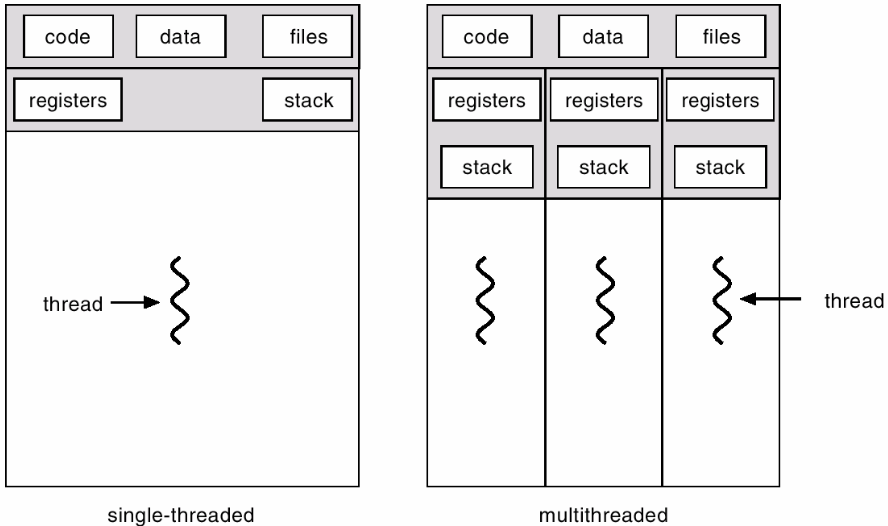
\includegraphics[width=0.9\textwidth]{figure/thread_single_vs_multi.png}
\end{frame}


\begin{frame}[fragile]
  \frametitle{2.7.1 线程的的基本概念(1)}
  1. 线程的优势:
  \begin{easylist} \easyitem
    & 响应速度(Responsiveness)
    && 减少并发执行时的时空开销,进程的创建、撤消、切换较费时空,因它既是调度单位,又是资源拥有者。

    & 资源共享(Resource Sharing)
    && 线程是系统独立调度和分派的基本单位,其基本上不拥有系统资源,只有少量资源
    (寄存器,栈…),但共享其所属进程所拥有的全部资源。
    
    & 充分利用多核/多处理器的硬件性能
    (Utilization of MP \& Multicore Architectures)
  \end{easylist}
\end{frame}


\begin{frame}[fragile]{2.7.1 线程的基本概念(2)}
  \begin{easylist} \easyitem
    & 2.线程的属性
    && 轻型实体
    && 独立调度和分派的基本单位
    && 可并发实体
    && 共享进程资源
    & 3.线程的状态
    && 状态参数
    &&& 寄存器状态、堆栈、运行状态、优先级、线程专有存储器、
    &&& 信号屏蔽
    && 线程的运行状态 
    &&& 就绪、执行、阻塞
  \end{easylist}
\end{frame}

\begin{frame}[fragile]{2.7.1 线程的基本概念(3)}
  \begin{easylist} \easyitem
    & 4.线程的创建和终止
    && 初始化线程
    & 5.多线程中的进程
    && 进程是拥有系统资源的基本单位,但不再是一个可执行的实体。
  \end{easylist}
\end{frame}

\begin{frame}[fragile]
  \frametitle{2.7.2 线程的类型}
  \begin{easylist}
  & 用户线程(User-level thread)
  && Thread management done by user-level threads library

  && 三种常见的用户线程
  &&& POSIX Pthreads
  &&& Win32 threads
  &&& Java threads
  
  & 内核线程(Kernel-Level Thread)
  && Supported by the Kernel
  &&& Windows XP/2000 ...
  &&& Linux
  &&& Mac OS X
  \end{easylist}
\end{frame}

\begin{frame}[fragile]
  \frametitle{用户线程向内核线程的映射}
  目的:把用户线程转换为内核线程,从而由操作系统调度执行
  \begin{easylist}
    & Many to One
    && Solaris Green Threads
    && GNU Portable Threads

    & One to One
    && Windows
    && Linux
    && Solaris 9 and later
    
    & Many to Many
    && Solaris prior to version 9
    && Windows NT/2000 with the ThreadFiber package
  \end{easylist}
\end{frame}

\begin{frame}[fragile]
  \frametitle{Many-to-one Model}
  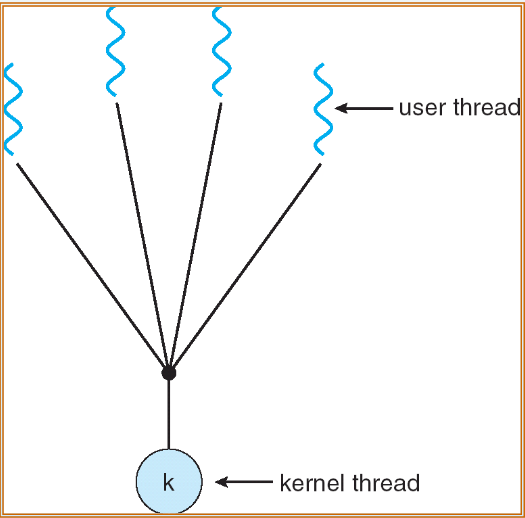
\includegraphics[width=0.6\textwidth]{figure/thread_many2one.png}
\end{frame}


\begin{frame}[fragile]
  \frametitle{One-to-one Model}
  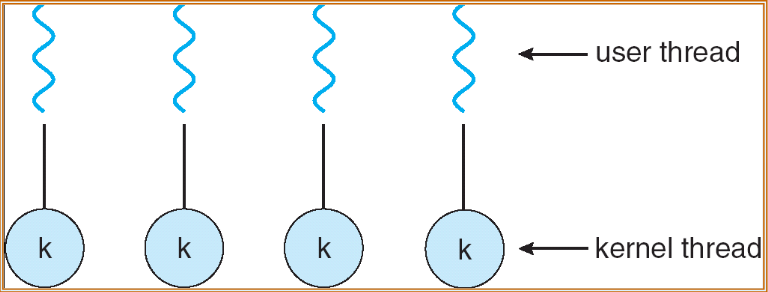
\includegraphics[width=0.9\textwidth]{figure/thread_one2one.png}
\end{frame}


\begin{frame}[fragile]
  \frametitle{Many-to-Many Model}
  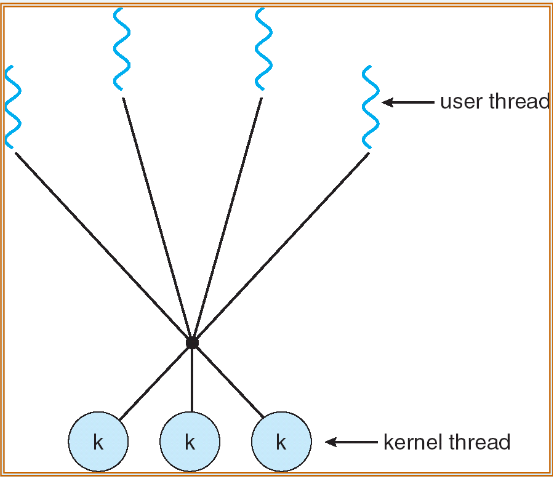
\includegraphics[width=0.6\textwidth]{figure/thread_many2many.png}
\end{frame}

\begin{frame}[fragile]{2.7.3 线程的同步和通信}
  \begin{easylist} \easyitem
    & 1.互斥锁
    && 阻塞方式 \\
    lock(mutex)\\
    访问\\
    unlock(mutex)\\

    && 非阻塞方式 \\
    if(trylock) then \\
    else \\
  \end{easylist}
\end{frame}

\begin{frame}[fragile]{2.7.3 线程的同步和通信}
  \begin{easylist} \easyitem
    & 2.条件变量
    && 用于线程的长期等待
    & 3.信号量机制
    && 私用信号量(private semaphore)
    &&& 作用域在一个进程中
    && 公用信号量(public semaphore)
    &&& 作用于多个进程间
  \end{easylist}
\end{frame}

\begin{frame}[fragile, allowframebreaks]{练习}
  \begin{enumerate}
  \item 进程的并发执行是指若干个进程( {\color{white} B}  ) \\
    A、同时执行          \\
    B、在执行的时间上是重叠的\\
    C、在执行的时间上是不可重叠的\\  
    D、共享系统资源 \\

  \item 若PV操作的信号量S初值为2,当前值为-1,则表示有( {\color{white} B}  )个等待进程。\\
    A、0个 \hspace{1cm}    B、1个 \hspace{1cm}   C、2个  \hspace{1cm}    D、3个

  \item 用PV操作管理临界区时,信号量的初值应定义为( {\color{white} C}  ) \\
    A、-1  \hspace{1cm}    B、0  \hspace{1cm}    C、1   \hspace{1cm}   D、任意值

  \item 用V操作唤醒一个等待进程时,被唤醒进程的状态变为( {\color{white} B}  ) \\
    A、等待  \hspace{1cm}  B、就绪   \hspace{1cm}  C、运行  \hspace{1cm}  D、完成

  \item ( {\color{white} D} )是一种只能进行P操作和V操作的特殊变量。(PV操作只能在
    ( {\color{white} D} )上操作) \\
    A、调度  \hspace{1cm} B、进程  \hspace{1cm} C、同步  \hspace{1cm} D、信号量

  \item 对于两个并发进程,设互斥信号量为mutex,若mutex=0,则({\color{white} B} ) \\
    A、表示没有进程进入临界区 \\
    B、表示有一个进程进入临界区 \\
    C、表示有一个进程进入临界区,另一个进程等待进入 \\
    D、表示有两个进程进入临界区 \\

  \item 临界区是({\color{white} C} ) \\
    A、一个缓冲区  \hspace{1cm} B、一段共享数据区  \\
    C、一段程序代码 \hspace{1cm}  D、一个互斥资源

  \item 信号量的物理意义是当信号量大于零时表示({\color{white} 可用资源数目} );
    当信号量小于零时,其绝对值为({\color{white} 因请求该资源而被阻塞的进程数目} )。

  \item 临界资源的概念是({\color{white} 一次仅允许一个进程访问的资源} ),而临界
    区是指({\color{white} 进程中访问临界资源的那段程序代码} )。

  \item 若一个进程已进入临界区,其它欲进入临界区的进程必须({\color{white} 等待} )。

  \item 用PV操作管理临界区时,任何一个进程在进入临界区之前应调用({\color{white}
      P} )操作,退出临界区时应调用({\color{white} V} )操作。

  \item 有m个进程共享同一临界资源,若使用信号量机制实现对临界资源的互斥访问,则信
    号量的变化范围是({\color{white} [-(m-1),1]} )。

  \item 操作系统中,对信号量S的P原语的定义中,使进程进入相应等待队列等待的条件是({\color{white} S<0} )。

  \item 如果信号量的当前值为-4,则表示系统中在该信号量上有({\color{white} 4} )个等待进程。

  \item 并发进程之间的基本关系是({\color{white} 互斥} )或({\color{white} 同步} )。
    其中({\color{white} 互斥} )是指进程之间的一种间接的关系。

  \end{enumerate}
\end{frame}



\begin{frame}[fragile]{本章作业及延伸阅读}
  \begin{easylist} \easyitem
    & 作业:操作系统同步之信号量机制

    根据文章介绍,实现并进行体验。https://zhuanlan.zhihu.com/p/34410587

    要求:以Markdown格式交作业,包括但不限于以下部分:

    && 整个测试流程及代码
    && 心得体会
    && 个人信息

    & 阅读(不用交):关于现代CPU,程序员应当更新的知识:

    http://www.iteye.com/news/30978
  \end{easylist}
\end{frame}



\begin{frame}[fragile]{}
 ~ 
\begin{center}
  --- END ---
\end{center}

\end{frame}
